

\section{Desarrollo}

En este informe se detalla el procedimiento seguido para el procesamiento de datos, el cual es crucial para su posible replicación futura. Este procedimiento incluye la obtención de imágenes, el uso de diferentes índices espectrales, y la clasificación de superficies mediante técnicas avanzadas de análisis de datos, todo orientado a extraer la información necesaria para un método numérico concreto de la bibliografía. La resolución matemática del modelo se proyecta para el futuro.

El código utilizado para llevar a cabo estos procesos se encuentra disponible públicamente en \href{https://github.com/justog220/TIF-Geomatica/}{GitHub} . Esta plataforma facilita la accesibilidad y la replicabilidad de los métodos utilizados, promoviendo la transparencia y la reutilización de los recursos desarrollados durante el proyecto.

\subsection{Área de estudio}

Para este estudio, se utilizaron datos recolectados a partir de la utilización de ovitrampas por parte de un proyecto de la Facultad de Ingenieria de la Universidad Nacional de Entre Ríos en Oro Verde, Entre Ríos, Argentina. El área de interés se definió mediante un procesamiento en Python, utilizando las bibliotecas Folium y Pandas. Este enfoque nos permitió generar gráficos detallados que representan los puntos geográficos con información sobre la densidad de mosquitos registrada experimentalmente. En la siguiente imagen (\figurename \ref{fig:ovitrampas}), se muestra la salida de este procesamiento, con un marcador representando cada ovitrampa.
	
\begin{figure}[H]
	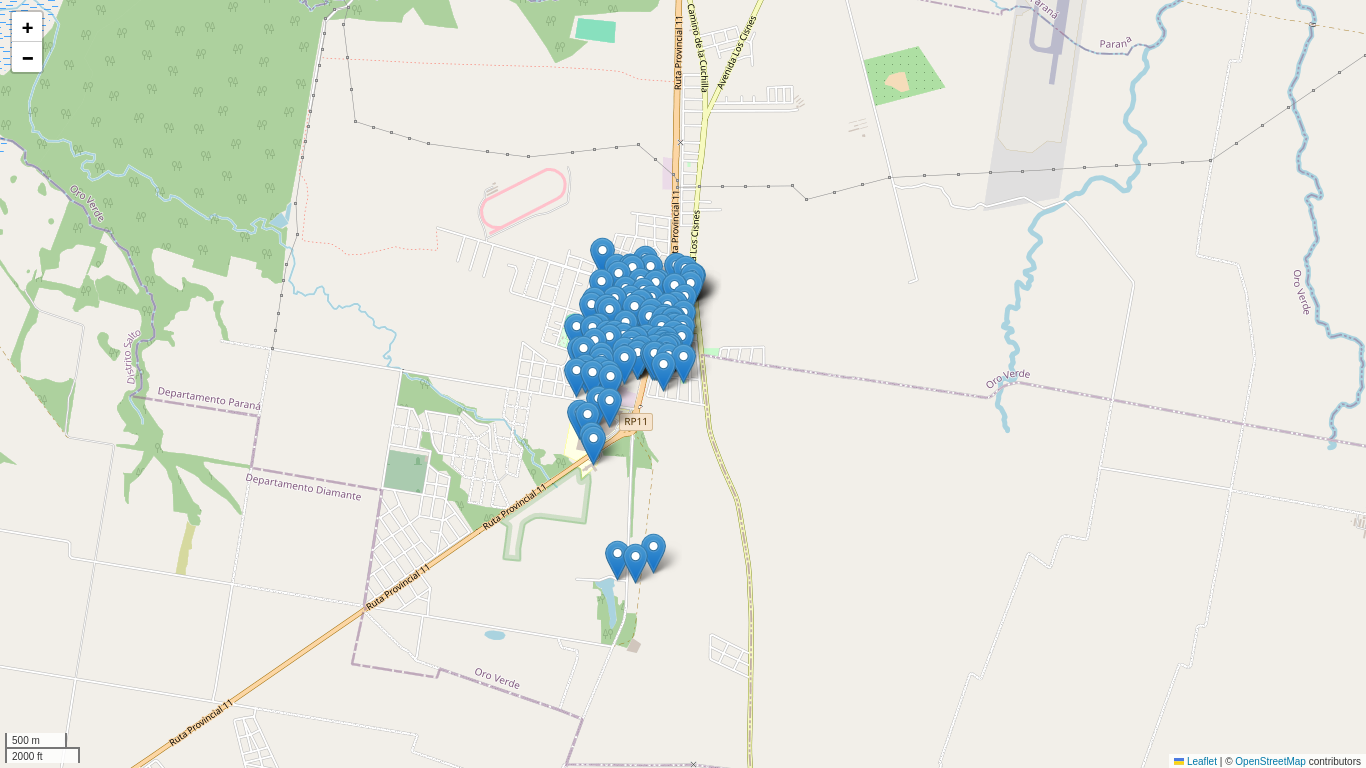
\includegraphics[width=0.7\textwidth]{ovitrampas.png}
	\centering
	\caption{Posiciones de ovitrampas en Oro Verde.}
	\label{fig:ovitrampas}
	
\end{figure}

A partir de estos marcadores, se extendió el procesamiento de los datos definiendo un cuadrado que encierra a todos los puntos con un margen adicional de 1km (\figurename \ref{fig:ovitrampas-ROI}). Esta delimitación nos permitió enfocarnos en el área específica para la cuál tenemos datos, es decir, nuestra región de interés (ROI, Region of Interest).

\begin{figure}[H]
	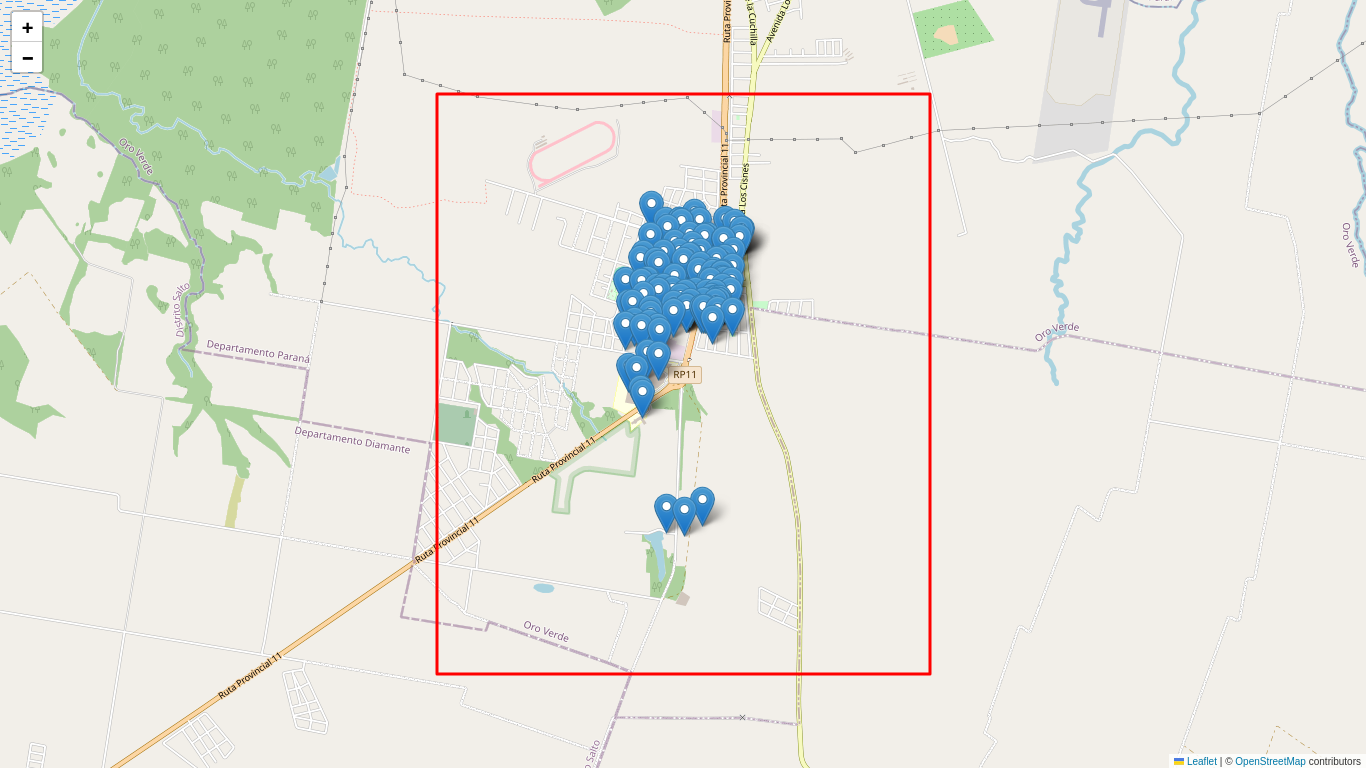
\includegraphics[width=0.7\textwidth]{ovitrampasConROI.png}
	\centering
	\caption{Posiciones de ovitrampas en Oro Verde con ROI delimitada.}
	\label{fig:ovitrampas-ROI}
	
\end{figure}

%% Podría ser buena idea agregar una foto del área de interés desde distintas perspectivas, una en la proyección mundial, otra en el mapa y después directamente la imágen.


\subsection{Obtención de imágenes}

Para el análisis, se utilizaron imágenes satelitales provenientes de Landsat 8, las cuales se obtendrán a través del Earth Explorer del USGS (United States Geological Survey) \parencite{noauthor_earthexplorer_nodate}¸. Estas imágenes, con un nivel de análisis L2, propocionan la información necesaria para estudiar la densidad de mosquitos en el área de interes a través de distintas técnicas.

\subsubsection{Dispositivo de sensado}

El Landsat 8 es un satélite de observación terreste que forma parte del Programa Landsat, administrado por el USGS y la NASA \parencite{noauthor_landsat_2021}. Este satelite consta de dos sensores principales:
\begin{itemize}
	\item OLI (Operational Land Imager)
	\item TIRS (Thermal Infrared Sensor)
\end{itemize}

A su vez, cada uno de estos sensores posee diversas bandas. Estas son listadas en la tabla \ref{table:landsat}.
\onehalfspacing

\begin{table}[H]
\begin{center}
	\begin{tabular}{|c | c | c|} 
		\hline
		\textbf{Banda} & \textbf{Longitud de onda ($\mu$)} & \textbf{Resolución espacial ($m$)}\\
		\hline
		1 - Coastal/Aerosol & 0.435-0.451 & 30 \\
		\hline
		2 - Azul & 0.452-0.512 & 30 \\
		\hline
		3 - Verde& 0.533-0.590 & 30 \\
		\hline
		4 - Roja & 0.636-0.673 & 30 \\
		\hline
		5 - NIR & 0.851-0.879 & 30 \\
		\hline
		6 - SWIR-1 & 1.566-1.651 & 30 \\
		\hline
		7 - SWIR-2 & 2.107-2.294 & 30 \\
		\hline
		8 - Pancromático & 0.503-0.676 & 15 \\
		\hline
		9 - Cirro & 1.363-1.384 & 30 \\
		\hline
		10 - TIR-1 & 10.60-11.19 & 100 \\
		\hline
		11 - TIR-2 & 11.50-12.51 & 100 \\
		\hline
	\end{tabular}
\end{center}
\caption{Tabla con información sobre las diferentes bandas que capta el Landsat 8}
\label{table:landsat}
\end{table}
\singlespacing

Para este estudio es muy relevante la diversidad de bandas espectrales, permitiendo analizar diversas características del terreno. Esta información, combinada con los datos de las ovitrampas, proporciona una visión integral y detallada del entorno.

%% TODO: desarrollar la comparativa con Landsat 5 que es el utilizado en el trabajo.

%% ADD PATH and ROW
\subsubsection{Análisis visual}

Como se mencionó previamente, se analizó la disponibilidad de imágenes a través de EarthExplorer. Se seleccionó la región de interés en esta plataforma y se estableció un rango de fechas según la disponibilidad de datos, comenzando con datos de  octubre de 2017. Se identificaron dos opciones de pasada del Landsat 8: una del path 227 y otra del 226, ambas para row 82. Estas opciones fueron marcadas en el mapa para evaluar la cobertura del área que proporcionaba cada una, como se muestra en \figurename \ref{fig:paths-rows}

\begin{figure}[H]
	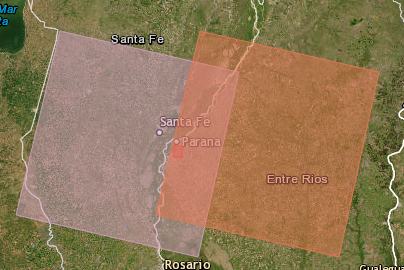
\includegraphics[width=0.7\textwidth]{pathsrows.png}
	\centering
	\caption{Opciones de cobertura.}
	\label{fig:paths-rows}
	
\end{figure}

Finalmente, se decidió utilizar la opción de la izquierda, ya que en la opción de la derecha, Oro Verde se encuentra sobre el borde de la imagen, lo que limitaría la capacidad de ampliar la región de interés. Por lo tanto, se procedió a la descarga de las imágenes correspondientes a la fecha de interés, utilizando el path 227 y el row 82.

Una vez obtenidos los datos de sensado de interés, se procedió a realizar un análisis visual detallado de la región utilizando el software QGIS \parencite{noauthor_qgis_nodate}. Este proceso incluyó la superposición de bandas espectrales como capas ráster y de los datos de coordenadas de las ovitrampas como vectores.

\subsection{Procesamiento de imágenes}


Con el objetivo de reducir el costo computacional y evitar el desperdicio de recursos, se procedió a definir un polígono delimitado por las coordenadas del área de interés. Este proceso incluyó la conversión de las coordenadas de las ovitrampas desde EPSG:4326 a EPSG:32620, seguido de la creación de un archivo de polígono con extensión \textit{.shp}.

Una vez que se estableció correctamente el archivo de polígono, se realizó una verificación visual utilizando QGIS para validar los cálculos (\figurename \ref{fig:polygon}). Posteriormente, se implementó el recorte de todos los archivos \textit{.TIF} utilizando la herramienta \textit{gdalwarp} de \textit{GDAL} \parencite{frank_gdalwarp_nodate}. 


\begin{figure}[H]
	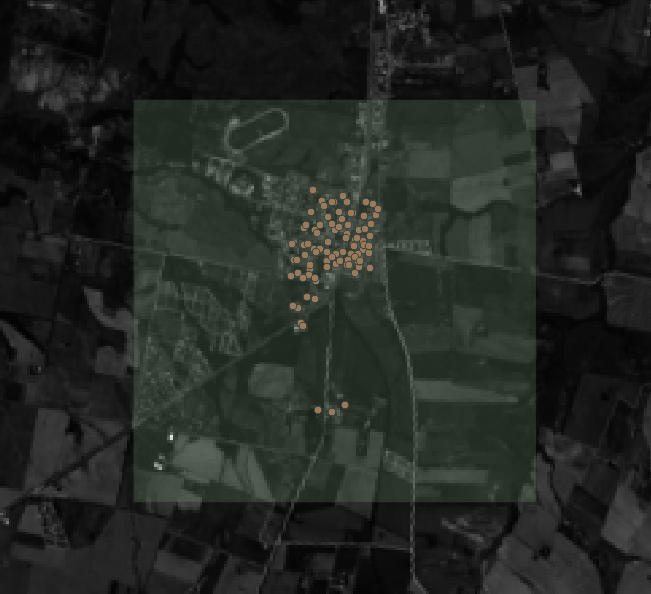
\includegraphics[width=0.7\textwidth]{polygon.png}
	\centering
	\caption{Polígono generado.}
	\label{fig:polygon}
\end{figure}

\subsection{Descripción del modelo}

El modelo presentado fue inicialmente propuesto por Raffy y Tran y ha sido aplicado en otras regiones de nuestro país, como en Salta \parencite{rotela_desarrollo_2012}. El modelo se describe matemáticamente de la siguiente manera:

$$\frac{\partial \rho(P,t)}{\partial t}=\bigtriangledown .(D_R \bigtriangledown \rho)-\bigtriangledown.(\rho D_W V)- \bigtriangledown . (\rho K_H \bigtriangledown H) + \alpha - \beta$$

Donde:

\onehalfspacing
\begin{center}
	\begin{tabular}{|c | c | c|} 
		\hline
		\textbf{Símbolo} & \textbf{Variable} & \textbf{Valor}\\
		\hline
		$$P$$ & Densidad de mosquitos & No homogéneo \\
		\hline
		$\alpha$  & Tasa de nacimientos & $6 (m^2/dia)$ \\
		\hline
		$\beta$  & Tasa de muertes             & 0.2 \\
		\hline
		$V$   & Velocidad Viento Superficie & No homogéneo \\
		\hline
		$K_H$   & Tensor de atracción         & 100 \\
		\hline
		$H$    & Campo de atracción          & No homogéneo \\
		\hline
		$D_R$   & Tensor de difusión          & No homogéneo / ver Tabla 2 \\
		\hline
		$D_W$   & Tensor de rugosidad         & No homogéneo / ver Tabla 2\\
		\hline
	\end{tabular}
\end{center}

Desglosando:

$$\frac{\partial \rho}{\partial t} (P,t)= Rozamiento(P,t)-Transporte(P,t)-Atraccion(P,t)+\alpha (P,t) - \beta (P,t¸)$$


Donde:
\doublespacing

$Rozamiento(P,t)=div[D_R (P,t) . \bigtriangledown \rho (P,t)]$

$Transporte(P,t)=[D_W (P,t) \vec{W} (P,t) . \bigtriangledown \rho (P,t)]$

$Atraccion(P,t) = div[K_H . \rho (P,t) . \bigtriangledown H (P,t)]$

\singlespacing

Con:

\begin{itemize}
	\item $\rho (P,t)$ = densidad de mosquitos
	\item $D_R (P,t)$ = tensor de rozamiento
	\item $D_W (P,t)$ = tensor de viento
	\item $W (P,t)$ = velocidad del viento
	\item $K_H$ = constante de atracción
	\item $H(P,t)$ = campo de atracción
	\item $\alpha (P,t)$ = razón de nacimientos
	\item $\beta (P,t)$ = razón de muertes
\end{itemize}

La resolución de estas ecuaciones se plantea como una proyección futura. En secciones posteriores se lleva a cabo la extracción de la información necesaria para aplicar el modelo en el área de estudio, como la medición de los parámetros de rugosidad y difusión ($D_W$ y $D_R$) a partir de la clasificación de superficies. La integración de estos datos permitirá la resolución del modelo, facilitando la predicción de la dinámica de las poblaciones de mosquitos en el área analizada.

\subsection{Cálculo de índices}

El cálculo de índices en geomática es una herramienta crucial para llevar a cabo diversos análisis y aplicaciones a partir de la transformación de la información contenida en las imágenes satelitales. Por esta razón, en este trabajo se utiliza una selección de algunos de estos índices que son relevantes para cumplir con el objetivo, a continuación se detallan aquellos utilizados.

\subsubsection{NDVI} \label{ndvi}

\paragraph{Cálculo}

El NDVI (Landsat Normalized Difference Vegetation Index) es usado para cuántificar cuán verde está la vegetación y es de utilidad a la hora de comprender la densidad de la vegetación \parencite{noauthor_landsat_nodate}.

Su cálculo de forma generalizada se lleva a cabo con la siguiente combinación de bandas:

$$NDVI=\frac{NIR-Red}{NIR+Red}$$

En el caso específicos de bandas de Landsat 8:

$$NDVI=\frac{Banda~5 - Banda~4}{Banda~5 + Banda~4}$$

En primer instancia, se llevó a cabo el cálculo con la función de calculadora ráster de QGIS. Sin embargo, luego se procedió a llevar a cabo una implementación en Python para su cálculo con el fin de tener el código necesario para automatizar su cálculo. Se evaluó una comparativa de los resultados obtenidos y el grado de precisión del cálculo era el mismo para ambos (\figurename \ref{fig:ndvi-comp})

\begin{figure}[H]
	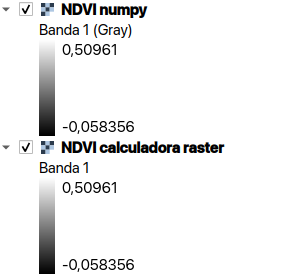
\includegraphics[width=0.3\textwidth]{ndviComp.png}
	\centering
	\caption{Comparativa de cálculos del NDVI.}
	\label{fig:ndvi-comp}
\end{figure}

\paragraph{Clasificación} \label{clasificacion}

Para la clasificación del tipo de vegetación en base al NDVI se consideraron cuatro clases: 1) Suelo expuesto, 2) Vegetación baja, 3) Vegetación alta; las cuales se etiquetaron con el siguiente criterio (\tablename    \ref{table:ndvi-criterio}): 

\onehalfspacing
\begin{table}[H]
\begin{center}
	\begin{tabular}{|c | c |} 
		\hline
		\textbf{Rango} & \textbf{Tipo}\\
		\hline
		Suelo expuesto & $0.0-0.25$ \\
		\hline
		Vegetación baja & $0.25-0.4$ \\
		\hline
		Vegetación alta & $> 0.4$ \\
		\hline
	\end{tabular}
\end{center}
\caption{Criterio de clasificación en base al NDVI.}
\label{table:ndvi-criterio}
\end{table}
\singlespacing

\subsubsection{NDWI}

El Índice Normalizado de Diferencia de Agua (NDWI) se emplea para destacar áreas de agua en una imágen captada por un satélite. Se utiliza principalmente para la detección y monitoreo de masas de agua \parencite{noauthor_ndwi_2021}. 

\paragraph{Cálculo}

El cálculo de este índice se lleva a cabo a partir de las bandas verdes y de infrarrojos cercanos, respetando la siguiente fórmula:

$$NDWI = \frac{Green - NIR}{Green + NIR}$$

Reformulando teniendo en cuenta la información correspondiente a las bandas del Landsat 8:

$$NDWI = \frac{Banda~3-Banda~5}{Banda~3+Banda~5}$$

El cálculo de este índice se realizo de la misma forma que en la sección \ref{ndvi}.


\paragraph{Clasificación} 

A las clases descritas en \ref{clasificacion}, se añade una nueva que representa cuerpos de agua. Se define como cuerpos de agua aquellos puntos con un valor de $NDWI$ superior a cero.

\subsubsection{NDBI}

\parencite{zha_use_2003}.

\paragraph{Cálculo}

El cálculo de este índice se lleva a cabo a partir de las bandas verdes y de infrarrojos cercanos, respetando la siguiente fórmula:

$$NDBI = \frac{SWIR1 - NIR}{SWIR1 + NIR}$$

Reformulando teniendo en cuenta la información correspondiente a las bandas del Landsat 8:

$$NDBI = \frac{Banda~6-Banda~5}{Banda~6+Banda~5}$$

El cálculo de este índice se realizo de la misma forma que en la sección \ref{ndvi}.

\subsubsection{NDBaI}

El índice NDBaI, o Índice Normalizado de Diferencia de Bareness y Albedo Integrado combina información sobre la ausencia de vegetación (bareness) y la reflectancia de la superficie (albedo) \parencite{hongmei_zhao_use_2005}s. Es útil para identificar áreas sin vegetación y evaluar la reflectancia de la superficie, proporcionando información complementaria en estudios de cobertura del suelo.

\paragraph{Cálculo}

$$NDBaI=\frac{SWIR1-TIRS1}{SWIR1+TIRS1}$$

Para las bandas específicas del Landsat 8, la fórmula se ajusta a:

$$NDBaI=\frac{Banda~6-Banda~10}{Banda~6+Banda~10}$$

\subsubsection{NDMI}

El Índice Normalizado de la Diferencia de Humedad (NDMI) se utiliza para evaluar la humedad en la superficie terrestre utilizando información de las bandas de infrarrojo cercano (NIR) e infrarrojo medio (SWIR1). Es especialmente útil para detectar y monitorear la presencia y cambios en la humedad del suelo y la vegetación, siendo aplicable en estudios ambientales y de recursos naturales.

\paragraph{Cálculo}

$$NDMI=\frac{NIR-SWIR1}{NIR+SWIR1}$$

La fórmula para calcular el NDMI en el contexto de Landsat 8 es la siguiente:

$$NDMI=\frac{Banda~5-Banda~6}{Banda~5+Banda~6}$$

\subsection{Clasificación de superficies}

Habiendo definido claramente los tipos de superficie a identificar y los criterios para determinarlos, se llevó a cabo la clasificación de los puntos del ráster siguiendo la secuencia lógica ya desarrollada de evaluación de índices. Todos los procesamientos relevantes para llevar a cabo este cometido se realizaron con Python y módulos propios de este lenguaje.

\begin{figure}[H]
	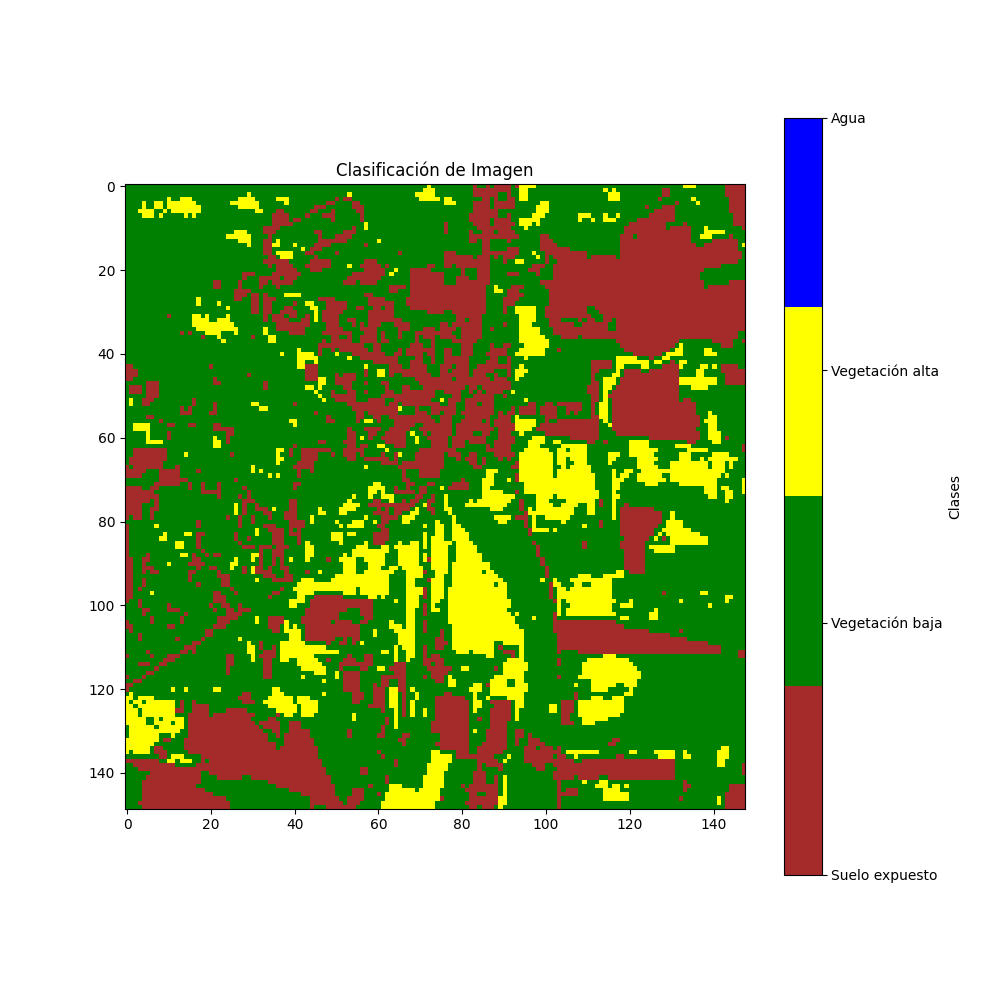
\includegraphics[width=0.7\textwidth]{clasificacion.png}
	\centering
	\caption{Capa con la clasificación para las distintas clases.}
	\label{fig:clasificacion}
\end{figure}

\subsection{Campo de atracción} \label{campo-de-atraccion}

El campo de atracción es un ráster del tamaño del área de interés, el valor de un pixel se determina por la densidad de píxeles que representan viviendas en su entorno cercado. Cuando un píxel contiene una vivienda (es decir, una fuente de hematofuentes) y está rodeado por una ventana de 90x90 metros (3 píxeles) que contiene exclusivamente viviendas el valor de atracción es máximo, estableciéndose en 1. En contraste, un píxel que no contiene viviendas y está rodeado por áreas que no incorporan hematofuentes obtiene un valor de atracción nulo \parencite{rotela_desarrollo_2012}. 

\subsubsection{Identificación de viviendas}

La identificación precisa de viviendas es fundamental para la determinación del campo de atracción en el análisis de datos geospaciales. Inicialmente, se empleó únicamente el NDBI como criterio para clasificar áreas con posibles viviendas. 

La validación de esta clasificación se llevó a cabo mediante un análisis visual en QGIS y un conocimiento profundo del área de estudio (ver \figurename \ref{fig:comparativa-ndbi}), se observó que el enfoque no logró identificar adecuadamente las zonas urbanas completas. Además, algunas áreas rurales fueron incorrectamente clasificadas como urbanas, indicando una falta de precisión en la distinción entre áreas construidas y no construidas.

\begin{figure}[!tbp]
	\begin{subfigure}[b]{0.49\textwidth}
		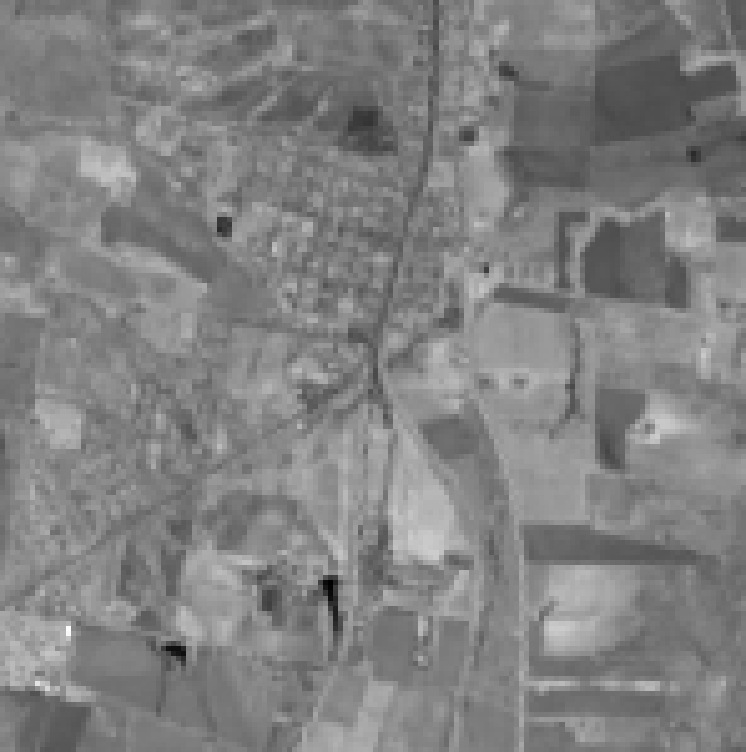
\includegraphics[width=\textwidth, height=\textwidth]{ndbiComp.png}
		\caption{Banda 5 del área de interés.}
		\label{fig:f1}
	\end{subfigure}
	\hfill
	\begin{subfigure}[b]{0.49\textwidth}
		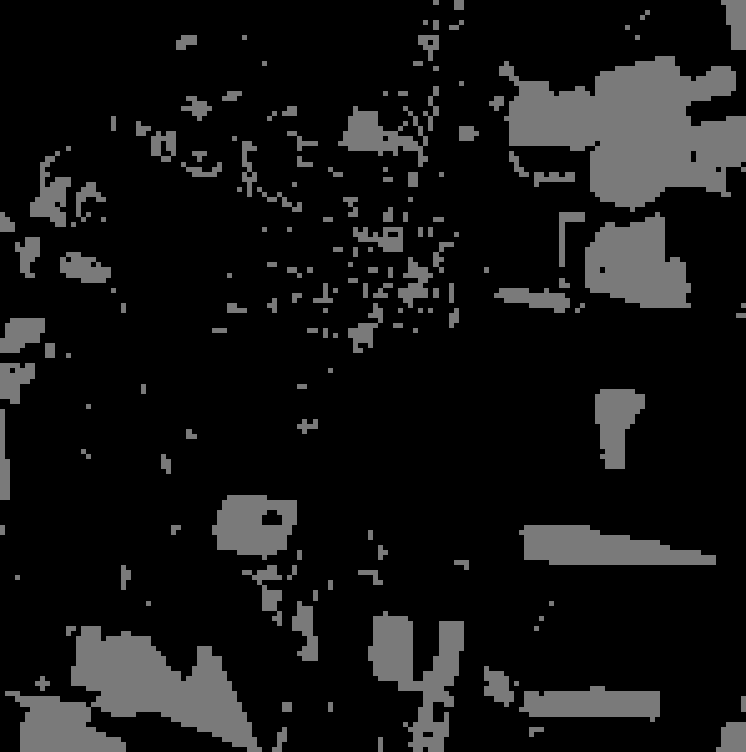
\includegraphics[width=\textwidth, height=\textwidth]{ndbi.png}
		\caption{$NDBI$ positivo como vivienda.}
		\label{fig:f2}
	\end{subfigure}
	\caption{Comparativa de la clasificación con el área de interés.}
	\label{fig:comparativa-ndbi}
\end{figure}

Con esta información sobre la mesa, se tomó la decisión de implementar una clasificación no supervisada utilizando el algoritmo de K-Means. Este enfoque fue elegido para mitigar posibles sesgos introducidos anteriormente y mejorar la precisión en la identificación de áreas urbanas y rurales. Se integraron diversos índices, incluyendo NDBI, NDVI, NDMI y NDBaI, con el objetivo de capturar múltiples aspectos del entorno que podrían indicar presencia de viviendas y otras estructuras construidas.

Después de calcular cada uno de los índices, se empleó el NDVI para generar una máscara identificando así los píxeles que corresponden a áreas de vegetación.

\begin{figure}[H]
	\begin{subfigure}[b]{0.49\textwidth}
		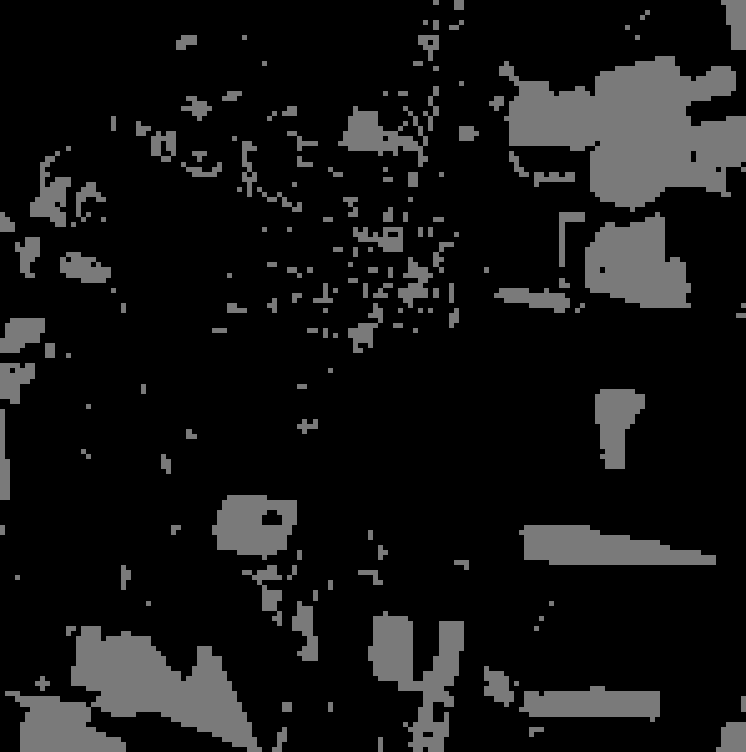
\includegraphics[width=\textwidth, height=\textwidth]{ndbi.png}
		\caption{Clasificación con $NDBI$.}
		\label{fig:ndbi-calculadora}
	\end{subfigure}
	\hfill
	\begin{subfigure}[b]{0.49\textwidth}
		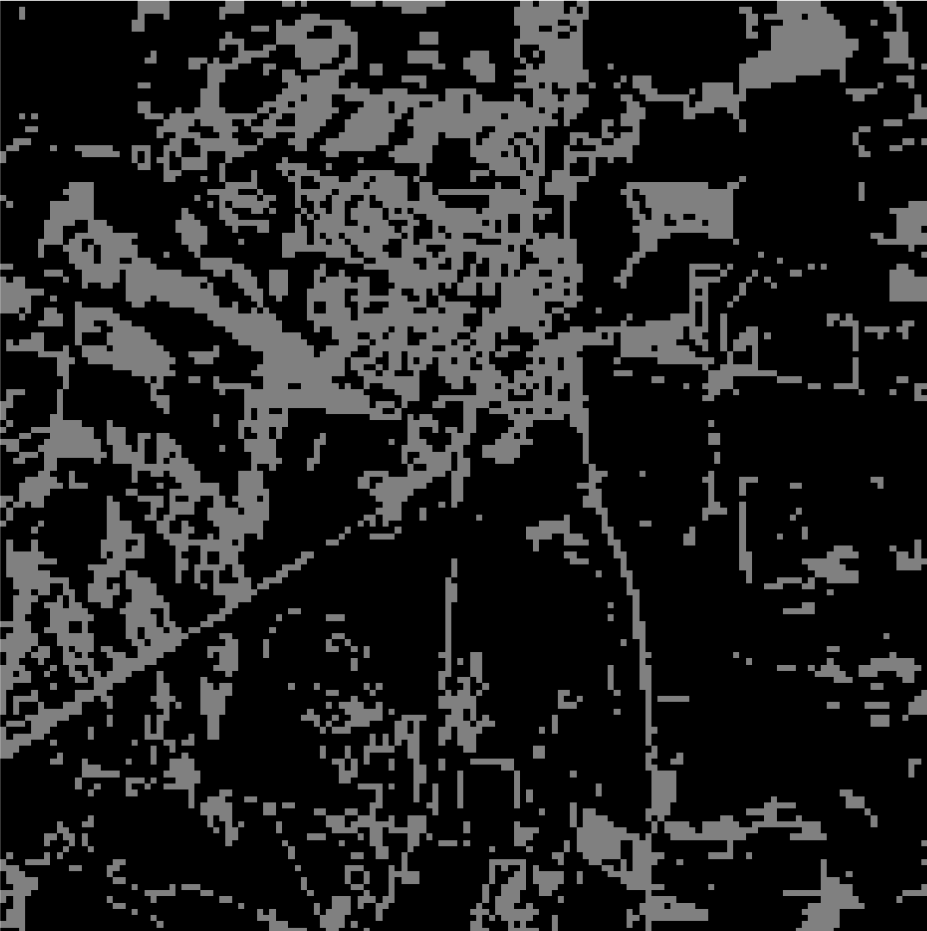
\includegraphics[width=\textwidth, height=\textwidth]{ndbikmeans.png}
		\caption{Clasificación con K-Means.}
		\label{fig:kmeans}
	\end{subfigure}
	\caption{Comparativa de la clasificación con el área de interés.}
	\label{fig:comparativa-ndbi-kmeans}
\end{figure}

Como se puede observar en la Figura \ref{fig:comparativa-ndbi-kmeans}, la clasificación resulta significativamente más precisa en comparación con el método anterior basado únicamente en NDBI. Esta mejora es evidente al considerar el conocimiento detallado del área de interés, donde ahora se logra una distinción más clara entre zonas urbanas y rurales. Por lo tanto, a partir de este punto, se adopta este criterio basado en la clasificación con K-Means para identificar y delimitar áreas que contienen viviendas en el estudio.

\subsubsection{Cálculo del campo de atracción}

Basandose en los fundamentos establecidos en la sección \ref{campo-de-atraccion}, se procedió a implementar el algoritmo para calcular el campo de atracción. En términos generales, este cálculo se realiza para cada punto según la siguiente fórmula:

$$Atraccion = 1 * \frac{Viviendas~vecinas}{Vecinas}$$

Este proceso genera una matriz de números decimales que reflejan la atracción que el vector sienten hacia cada píxel debido a la presencia de hematofuentes, variando de 0 a 1 (ver Figura \ref{fig:atraccion}).

\begin{figure}[H]
	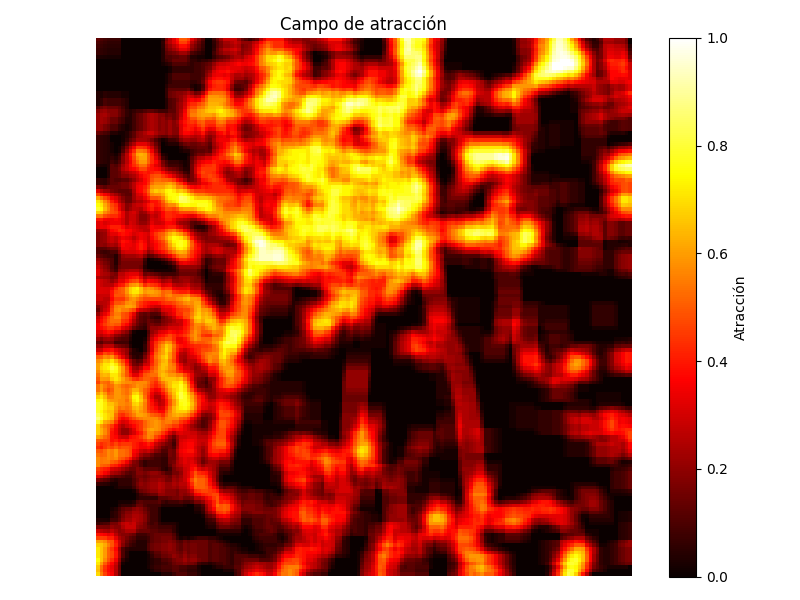
\includegraphics[width=0.7\textwidth]{campoDeAtraccion.png}
	\centering
	\caption{Campo de atracción para la región de interés.}
	\label{fig:atraccion}
\end{figure}

\subsection{Densidad inicial}

En esta subsección, se detalla el procedimiento utilizado para calcular la densidad inicial de huevos en el área de interés, empleando técnicas avanzadas de procesamiento de imágenes y análisis de datos geoespaciales.

\subsubsection{Lectura y procesamiento de datos}

El primer paso consistió en la lectura y procesamiento de los datos de entrada. Se utilizaron dos tipos de datos: una imagen rasterizada en formato TIF y un archivo CSV con coordenadas y conteos de huevos.

El archivo CSV contiene datos puntuales con coordenadas y conteos de huevos, los cuales se filtraron por una fecha específica a modo de ejemplo para enfocarse en un momento determinado del estudio, que se corresponde con aquella en la que más huevos se registraron.

\subsubsection{Interpolación gaussiana}

Para calcular la densidad espacial de los huevos, se empleó una técnica de interpolación basada en una función gaussiana bidimensional. La función gaussiana es una representación matemática que describe una distribución normal en dos dimensiones, caracterizada por su forma de campana:

\begin{equation}
	G(x, y) = \exp\left(-\frac{(x - x_0)^2 + (y - y_0)^2}{2\sigma^2}\right)
\end{equation}

Se utilizó esta función para modelar la distribución espacial de los huevos alrededor de cada punto de datos. 

\subsubsection{Visualización de resultados}

Finalmente, los resultados se visualizaron superponiendo el mapa de densidad calculado sobre la imagen TIF original. Esta visualización permite observar la distribución espacial de la densidad de huevos en la región de estudio (Figura \ref{fig:densidad}).

\begin{figure}[H]
	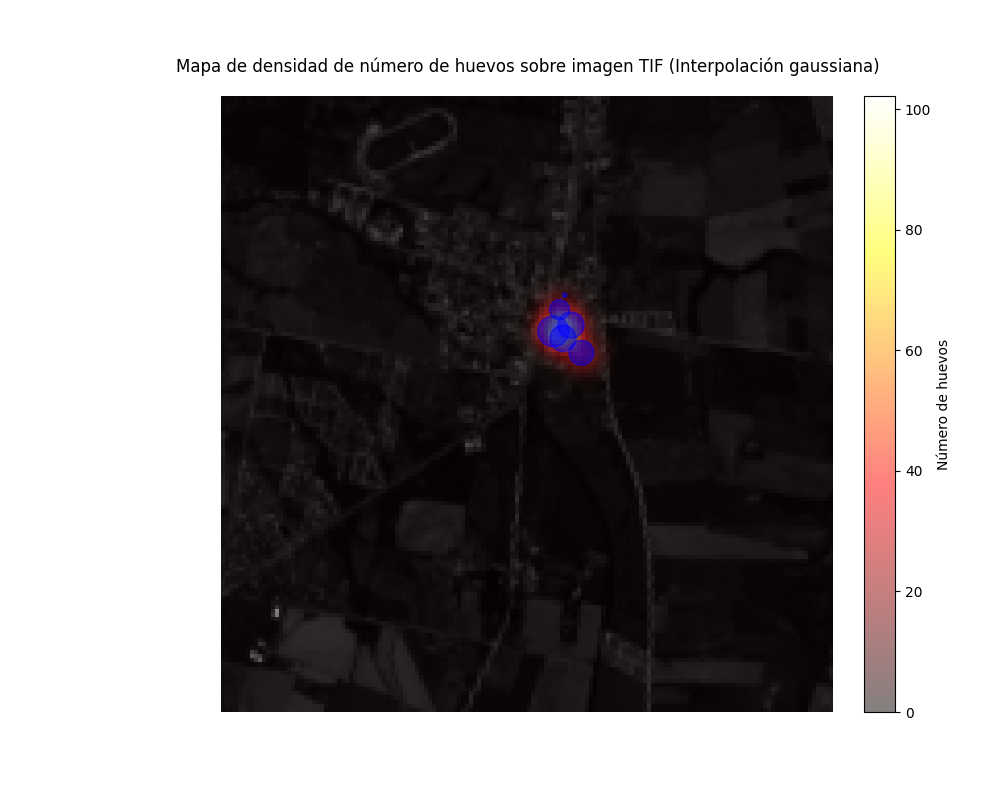
\includegraphics[width=\textwidth]{densidad.png}
	\centering
	\caption{Densidad inicial para la región de interés.}
	\label{fig:densidad}
\end{figure}


\subsection{Integración de módulos}

Habiendo desarrollado los módulos con las funcionalidades necesarias para obtener la información requerida por el modelo, se procedió a integrarlos para realizar desde el procesamiento inicial de imágenes hasta la generación de mapas de densidad.

\subsubsection{Preparación del entorno y recorte de imágenes}

El punto de partida es la preparación del entorno de trabajo con las carpetas utilizadas y el recorte de las imágenes raster, destinado a optimizar los recursos computacionales. Este paso asegura la extracción de áreas relevantes para análisis detallados.

\subsubsection{Cálculo de índices}

Recortadas las imágenes, se procede al cálculo de diversos índices espectrales, que proporcionaran, por ejemplo, información vital sobre la presencia de vegetación y/o humedad.

\subsubsection{Clasificación de suelo y urbanización}

Con los índices calculados, se lleva a cabo la clasificación de las clases. Permitiendo identificar y mapear distintas categorías como Suelo expuesto, Vegetación baja, Vegetación alta y Agua. Además, se realiza un análisis de la urbanización mediante agrupamientos no supervisado de los píxeles en base a los diversos índices calculados para ellos.

\subsubsection{Cálculo del campo de atracción y análisis de densidad}

Con las clasificaciones previas y los datos de ovitrampas se está en condiciones de llevar a cabo el cálculo del campo de atracción como se describió previamente y la estimación de la densidad incial de mosquitos. 

Este flujo de trabajo integrado y estructura facilita la interpretación de datos complejos y la extracción de características fundamentales para la aplicación posterior en el modelo matemático.